
\section{Descrição da Inovação}

A inovação no projeto EMMA é utilizar a robótica para realizar reparo e
revestimento \textit{in situ} em pás de turbinas de hidroelétricas, ou seja, sem
precisar desinstalar e remover as pás. A metodologia do processo é iniciada com o
ensecamento e entrada do corpo técnico ao circuito hidráulico. A metodologia
desenvolvida segue como explicado pelas imagens.

% \begin{figure}[H] 
% 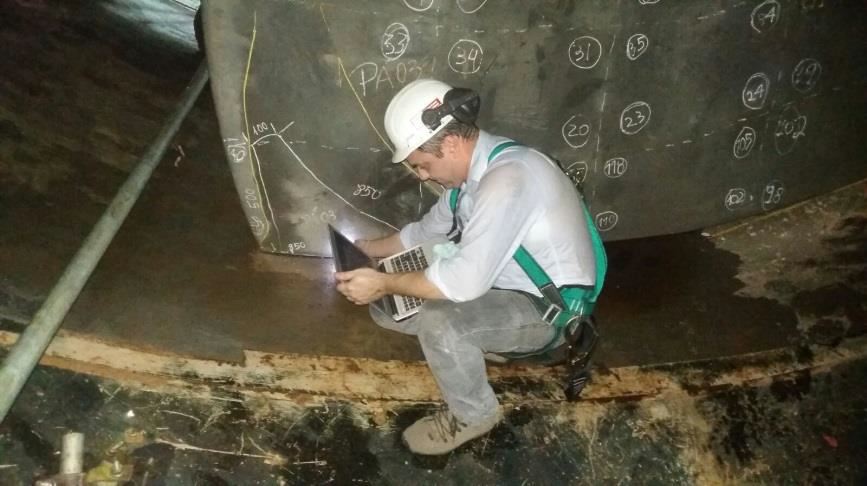
\includegraphics[width=0.9\linewidth, height=4cm]{figs/manolo} 
% \caption{A equipe técnica analisa a pá verificando o desgaste do coating
% existente e se existem danos a pá em si.}
% \label{fig:subim1}
% \end{figure}
% 
% \begin{figure}[H] 
% 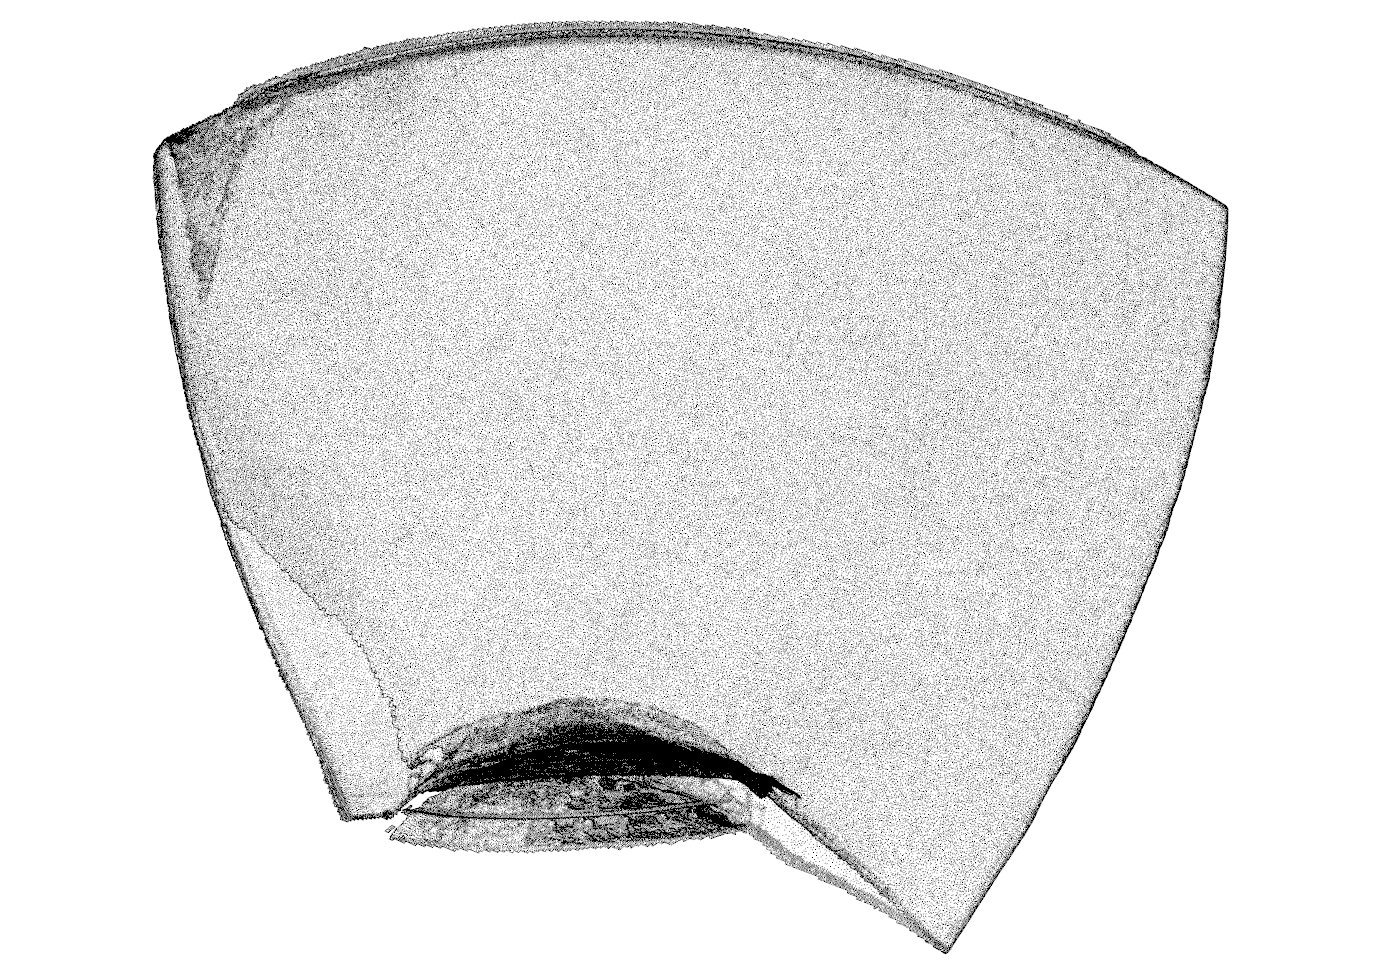
\includegraphics[width=0.9\linewidth, height=4cm]{figs/modelo_pa_faro}
% \caption{Dado a necessidade de reparo um laser scanner de metrologia é
% utilizado para mapear o dano com uma precisão de 2mm.}
% \end{figure}
% 
% \begin{figure}[H]
% 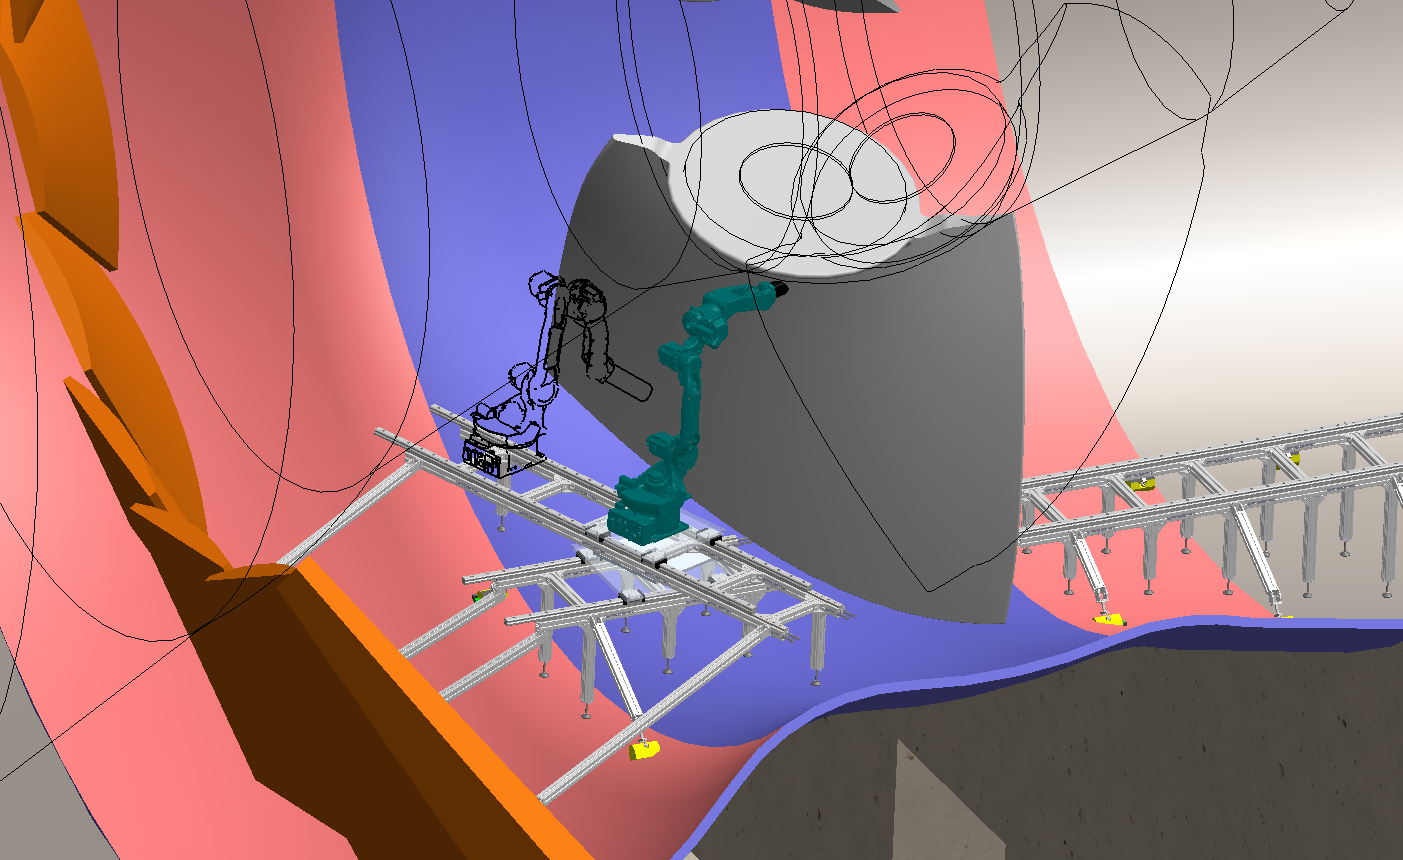
\includegraphics[width=0.9\linewidth, height=4cm]{figs/EMMA_Base_Secundaria_01} 
% \caption{Um trilho modular é instalado no ambiente e aconrado através de pinos
% magnéticos. O trilho é utilizado para levar o manipulador até a pá e movimentar
% o manipulador ao longo da área de trabalho.}
% \end{figure}
% 
% \begin{figure}[H]
% 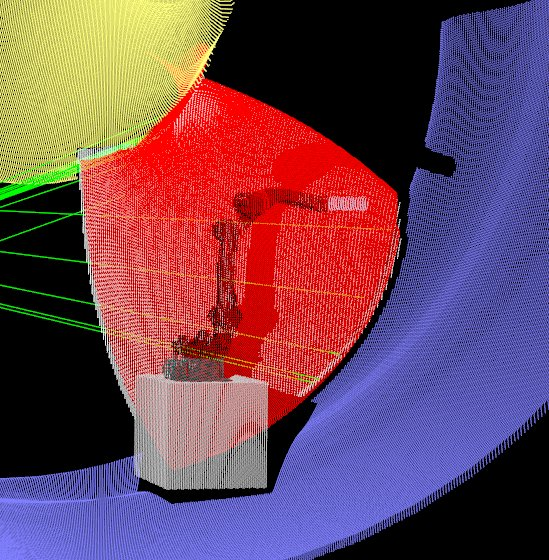
\includegraphics[width=0.9\linewidth, height=4cm]{figs/localizacao}
% \caption{Algoritmo de processamento de nuvens de pontos analisam um scan laser
% do ambiente e estimam a posição relativa entre o manipulador e a pá.}
% \end{figure}


\begin{figure}[H]
\begin{subfigure}{0.5\textwidth}
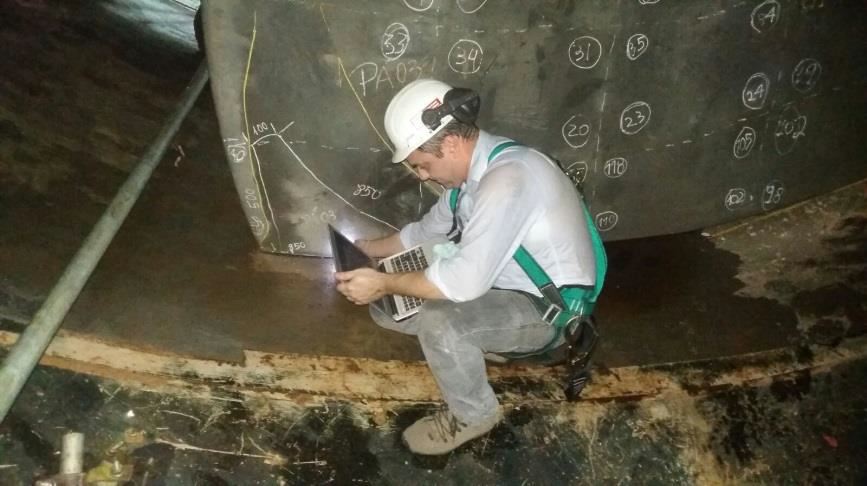
\includegraphics[width=0.9\linewidth, height=4.1cm]{figs/manolo}
\captionsetup{width=0.9\textwidth}
\caption{A equipe técnica analisa a pá verificando o desgaste do coating
existente e se existem danos a pá em si.}
\label{fig:subim1}
\end{subfigure}
~
\begin{subfigure}{0.5\textwidth}
\label{fig:subim2}
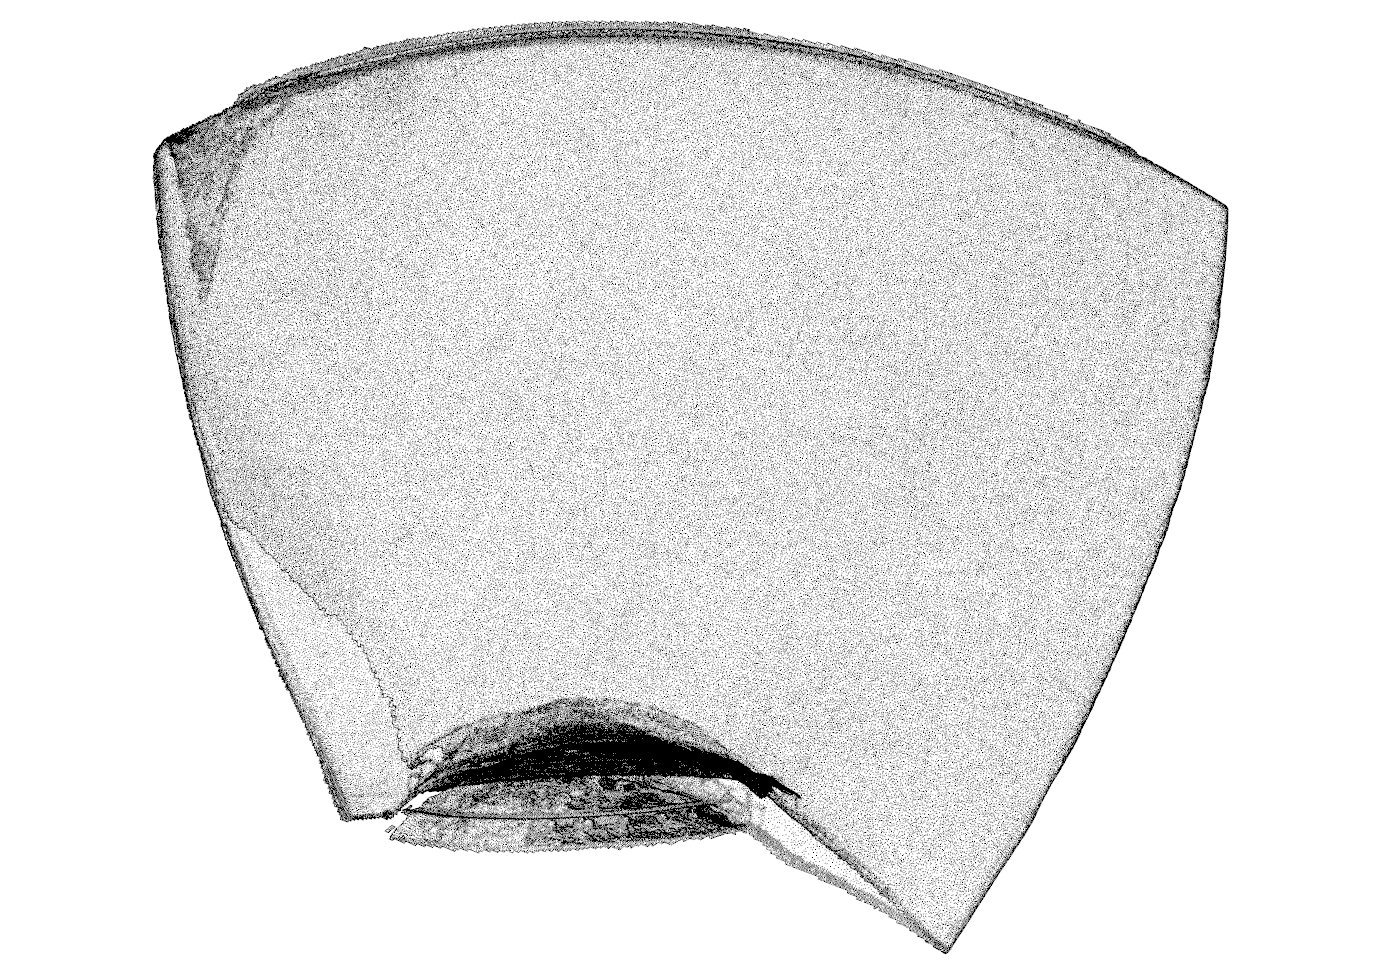
\includegraphics[width=0.9\linewidth, height=4.1cm]{figs/modelo_pa_faro}
\captionsetup{width=0.9\textwidth}
\caption{Dado a necessidade de reparo um laser scanner de metrologia é
utilizado para mapear o dano com uma precisão de 2mm.}
\end{subfigure}
 \label{fig:image2}
\end{figure}

\begin{figure}[H]
\ContinuedFloat
\begin{subfigure}{0.5\textwidth}
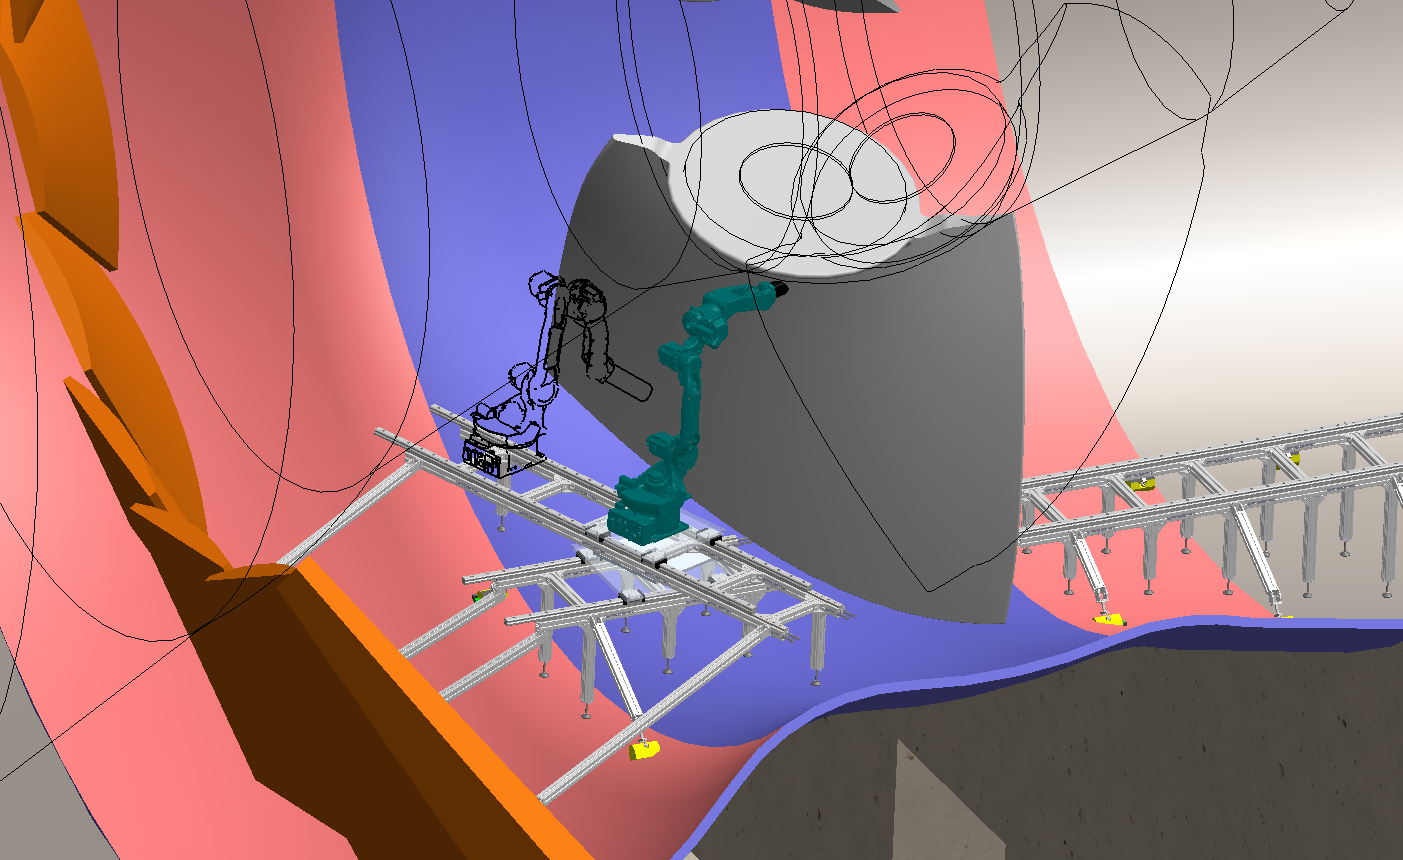
\includegraphics[width=0.9\linewidth,
height=4.1cm]{figs/EMMA_Base_Secundaria_01}
\captionsetup{width=0.9\textwidth}
\caption{Um trilho modular é instalado no ambiente e aconrado através de pinos
magnéticos. O trilho é utilizado para levar o manipulador até a pá e movimentar
o manipulador ao longo da área de trabalho.}
\end{subfigure}
~
\begin{subfigure}{0.5\textwidth}
\label{fig:subim2}
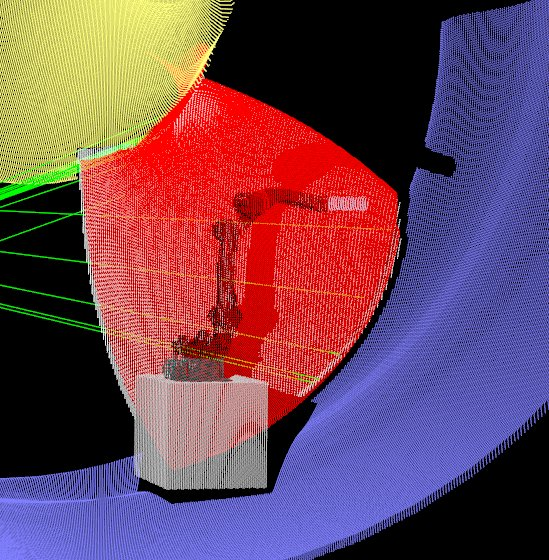
\includegraphics[width=\linewidth, height=4.1cm]{figs/localizacao}
\captionsetup{width=0.9\textwidth}
\caption{Algoritmo de processamento de nuvens de pontos analisam um scan laser
do ambiente e estimam a posição relativa entre o manipulador e a pá.}
\end{subfigure}
 \label{fig:image2}
\end{figure}


\begin{figure}[H]
\ContinuedFloat
\begin{subfigure}{0.5\textwidth}
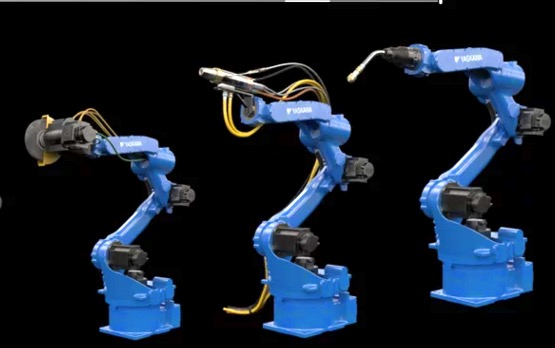
\includegraphics[width=0.9\linewidth, height=4.1cm]{figs/robots_evo} 
\captionsetup{width=0.9\textwidth}
\caption{O equipamento necessário para a tarefa, seja soldagem, esmerilhamento
ou coating é instalado no manipulador e o ambiente e superfície são preparados.}
\end{subfigure}
~~~
\begin{subfigure}{0.5\textwidth}
\label{fig:subim2}
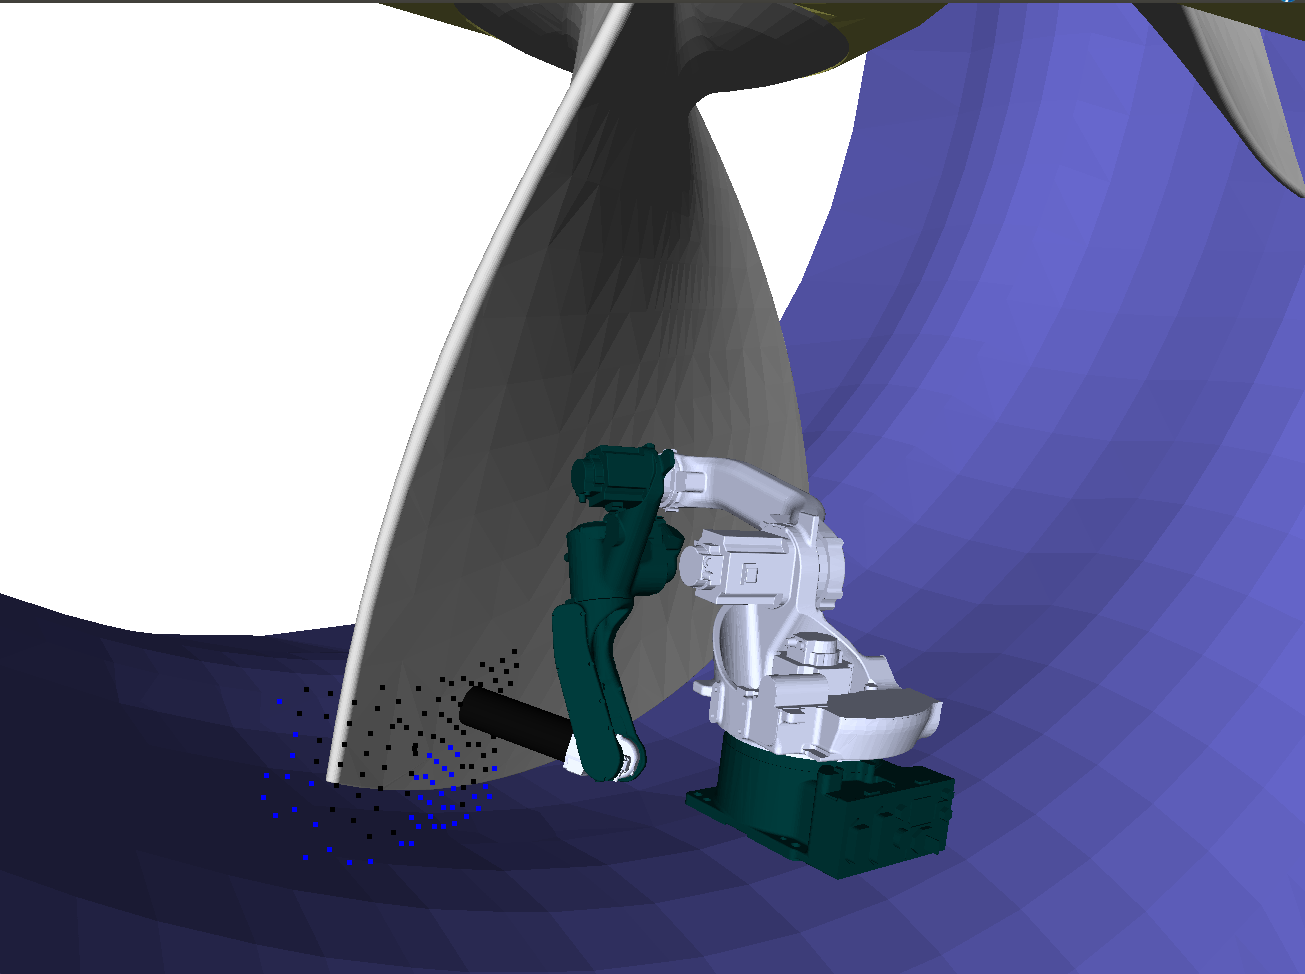
\includegraphics[width=0.9\linewidth, height=4cm]{figs/footleft}
\captionsetup{width=0.9\textwidth}
\caption{O algoritmo estima e executa a trajetória para a tarefa planejada.}
\end{subfigure}
 \label{fig:image2}
\end{figure}

O resultado do processo será uma pá restaurada e protegida, aumentando a
eficiência de geração e vida útil da mesma. 

\section{Motivação}

Desgastes por corrosão, erosão e abrasão em pás de turbinas de hidroelétricas
resultam em perda do perfil hidráulico, reduzindo assim a eficiência de geração.
O desgaste reduz também a vida útil da turbina, o tempo de operação entre
paradas de manutenção, assim como, aumentam os custos de manutenção e o tempo
necessário de parada de máquina para a realização do reparo. Logo, significa uma
perda da eficiência de geração, e por consequente um impacto econômico
significativo na operação.
A aplicação de revestimento aumenta a resistência do material contra os
desgastes, custando em torno de 20\% do valor de uma peça nova e representando
um aumento da vida útil em mais de 300\%. Entretanto, dados as limitações da
tecnologia atual, só é possível aplicar o revestimento em bancada, logo, antes
da instalação das pás. Logo, o desenvolvimento tecnológico que possibilite
reaplicar a camada de revestimento dentro do circuito hidráulico resultaria em
um ganho significativo na geração e redução dos custos de operação.
Antes de aplicar o revestimento é necessário reparar a pá recuperando o perfil
hidráulico da mesma, quanto maior a precisão da recuperação do perfil hidráulico
maior a eficiência de geração. Logo, a robótica se torna a ferramenta ideal para a tarefa.

\section{Objetivo}

O objetivo geral do projeto é desenvolver e testar uma metodologia que permita
utilizar a robótica para reparar e revestir pás instaladas em circuitos hidráulicos.

Os objetivos específicos são determinar as metodologias: 

\begin{itemize}
  \item definir o manipulador ótimo para cada hidroelétrica; 
  \item movimentar o manipulador dentro do circuito hidráulico;
  \item estimar a posição do manipulador com relação ao meio;
  \item material e técnica de coating e reparo; 
  \item preparar o meio e superfície;
  \item logística para instalar um sistema robótico no circuito hidráulico;
  \item determinar os riscos associados;
  \item planejar e executar a manipulação;
  \item representar as diferentes informações do processo para um operador;
  \item verificar as perdas de carga do processo de revestimento;
  \item integrar e utilizar as diversas ferramentas;
  \item mapear o perfil hidráulico e medir os danos.
\end{itemize}

\section{Originalidade}

Não existe nenhuma solução ou estudo realizado sobre a aplicação de revestimento
dentro do circuito hidráulico sem desinstalar as pás da turbina. A aplicação de
revestimento para proteção contra abrasão, cavitação, corrosão e erosão em peças
de turbinas de hidrelétricas realizado atualmente é limitada a trabalho em
bancada com a peça desinstalada. O desafio de realizar o trabalho de
revestimento dentro do circuito hidráulico se dá pela dimensão da escotilha de
acesso, que limita o tamanho do robô, pelo posicionamento do robô com relação a
pá da turbina, que se encontra a alguns metros do solo, pelo processo de
aplicação que requer velocidade constante utilizando uma pistola pesada e pelo
controle de temperatura e humidade necessários. Esta pesquisa é inovadora no
setor elétrico brasileiro e é um avanço com relação ao estado da arte.

\section{Aplicabilidade}

A metodologia desenvolvida no projeto  poderá ser aplicada na maioria das
hidroelétricas de médio ou grande porte. A metodologia determina o tamanho e
modelo de manipulador ótimo para o circuito hidráulico em questão, assim como,
qual material de coating a ser aplicado. A restrição para aplicação da tecnologia é
apenas dada pelo espaço entre as pás, em hidroelétricas de pequeno porte a
pistola de coating não cabe entre as pás. Logo, a abrangência é nacional,
entretanto com restrição de uso em pequenas unidades geradoras.

\section{Relevância}

A matriz geradora Brasileira é constituída em sua maioria por geração
hidráulica, com um grande número de centrais em rios tipos corredeiras que
possuem reservatórios pequenos. Neste tipo de rio não há tempo de sedimentação
das partículas sólidas na água, essas partículas sólidas, mesmo em quantidades
pequenas, geram um elevado nível de desgaste por erosão e cavitação. Logo, o
projeto é de relevância para o setor elétrico e para a nação, pois aumenta a
eficiência da matriz energética Brasileira, aumenta a disponibilidade da máquina
para geração e reduz os custos de manutenção, representando uma melhora
econômica e social.

\section{Capacitação}

A Pesquisa e Desenvolvimento (P\&D) tem como propósito fomentar o avanço
tecnológico e novas maneiras de desenvolver um tipos específicos de conhecimento
no país. O desenvolvimento do Projeto EMMA, no âmbito P\&D é um exemplo de como
a parceria entre agências do governo, empresa e universidades podem colaborar para
a capacitação tecnológica e o desenvolvimento de novas tecnologias.

O projeto EMMA possui 2 pesquisadores inscritos no mestrado, assim como um
inscrito na graduação.
Os temas são todos no campo da robótica, sendo a previsão de conclusão das dissertações
esperada para a fase 2 e fase 3 do EMMA. Os alunos de mestrado e seus
respectivos cursos são:

\begin{itemize}
  \item Estevão Fróes Ferrão, Programa de Engenharia Mecânica/COPPE, Rio de
  Janeiro, com o tema ``Controle de precisão de um manipulador robótico devido à
  flexibilidade e vibrações de uma base mecânica e do próprio manipulador, dadas
  suas cargas dinâmicas;
  %TODO Titulo e tema de mestrado ESTEVAO E JULIA
  \item Julia Ramos Campana, Departamento de Artes e Design, PUC, Rio de
  Janeiro, com o tema ``Métodos para o design de interfaces gráficas em
softwares de sistemas autônomos: um estudo de usabilidade e interação
humano-computador''.
 \item Felipe Guerin, Engenharia Mecânica, nível Graduação e Cursos Sequenciais
 na Universidade do Vale do Rio dos Sinos.
\end{itemize}
O projeto também proporcionou a elaboração e submissão de dois artigos
acadêmicos:

\begin{itemize}
  \item State of the art and conceptual design of robotic solutions for in situ
  hard coating of hydraulic turbines, Journal of Control, Automation and
  Electrical Systems (JCAE). Autores: Renan S. Freitas, Gabriel Alcantara C. S.,
  Eduardo Elael M. S., Estevão Fróes F., Ramon R. Costa;
  \item A Robotic System for in situ Hydropower Turbine Hard Coating, Congresso
  Brasileiro de Automática (CBA). Autores: Renan S. Freitas, Estevao F. Ferrão,
  Gabriel Alcantara C. S., Eduardo Elael M. S., Ramon R. Costa.
\end{itemize}

Os artigos se encontram, na íntegra, anexados a este relatório no apêndice
\ref{app:artigos}.



Para o comprimento dos requisitos de segurança, a equipe do projeto foi submetida à capacitação, nas
normas relevantes às situações encontradas no interior do circuito hidráulico. As certificações foram nas
seguintes normas:

\begin{itemize}
  \item NR10 - Segurança e Instalações e Serviços em Eletricidade;
  \item NR33 - Segurança e Saúde nos Trabalhos em Espaços Confinados;
  \item NR35 - Trabalho em Altura.
\end{itemize}

Seguem listados os pesquisadores que foram capacitados no curso
supracitado:

\begin{itemize}
  \item Estevão Fróes Ferrão, Programa de Engenharia Mecânica/COPPE;
  \item Gabriel Alcantara Costa Silva, Programa de Engenharia Elétrica/COPPE;
  \item Renan Sales de Freitas, Programa de Engenharia Elétrica/COPPE;
  \item Eduardo Elael de Melo Soares, Programa de Engenharia Elétrica/COPPE;
  \item Julia Ramos Campana, Departamento de Artes e Design, PUC, Rio de
  Janeiro;
  \item Gabriel Cogo, RIJEZA Indústria Metalúrgica.
\end{itemize}

% A pesquisa no projeto EMMA proporcionou a elaboração de dois artigos
% submetidos/publicados em revistas, abordando os seguintes tópicos: 
% 
% \begin{itemize}
%   \item Estado da arte e design conceitual de soluções robóticas para
%   revestimento de turbinas hidráulicas \textit{in situ} (State of the art and
%   conceptual design of robotic solutions for \textit{in situ} hard coating of
%   hydraulic turbines).
%   \item Solução Conceitual e estudo de viabilidade técnica para para
%   revestimento de turbinas hidráulicas \textit{in situ} (EMMA - A robotic
%   system for \textit{in situ} hydropower turbine hard coating).
% \end{itemize}

\section{Razoabilidade dos Custos}

Atualmente, após a instalação da Unidade Geradora (UG), não existe método
disponível para proteger a ogiva geradora contra os desgastes de sua utilização. Sendo,
infelizmente, a recuperação sempre o caminho e isso pode ser estimado entre 90 e
120 dias de UG parada. A frequência de paradas de recuperação variam dependendo
do tempo de operação da unidade geradora, material, tipo de bacia e etc. A única
certeza é que um dia será necessário. A aplicação de revestimento pode ser realizada
durante as paradas planejadas, sem perda de tempo de geração.
De acordo com \cite{calainho1999cavitaccao}, em média 5 unidades geradoras
apresentaram  cavitação a cada 24.071 horas de operação (2,7 anos), das 36 instalações analisadas. Logo, em Jirau a
aplicação do revestimento \textit{in situ} significaria em um aumento da
disponibilidade de geração de 600 dias a cada 2,7 anos, considerando turbinas de 75 MW de
potencia, seria equivalente a 1.080.000 MW a cada 2,7 anos.

Além do ganho de disponibilidade, estudos da Andritz
\footnote{\url{https://www.andritz.com/hy-hn19-en.pdf}}, demonstram que turbinas
revestidas possuem um ganho na eficiência de geração, aproximadamente em média de 2\% a
cada 30.000 horas, como ilustrado na figura \ref{fig:coating_graph}. Em Jirau,
isso significaria um ganho por turbina de 45.000 MW por turbina a cada 3,5 anos. Considerando a capacidade instalada de
50 turbinas, isso significaria 2.250.000 MW a cada 3,5 anos.

\begin{figure}[h!]
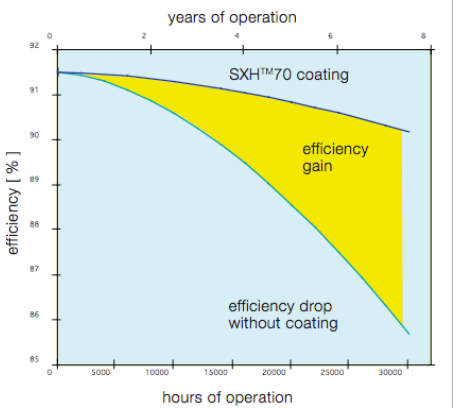
\includegraphics[width=0.8\textwidth]{figs/coating_graph}
\caption{Influência do coating na eficiência durante a operação com presença de
alta erosão abrasiva.}
\label{fig:coating_graph}
\end{figure}

\section{Metodologia adotada}

O projeto EMMA foi dividido em 3 fases, sendo cada fase um projeto distinto.
Cada fase avançando a tecnologia ao longo da cadeia de inovação. Na primeira
fase foi desenvolvido a metodologia/conceito. Na segunda fase será feito o
desenvolvimento experimental testando o sistema de coating. Na terceira fase, a
solução será expandida para incluir reparo e validar a tecnologia em
outras centrais hidroelétricas.

Ao início da primeira fase não se sabia se existiria uma solução para o
problema. Os requisitos de acesso, operação e coating são extremamente
limitantes. A metodologia adotada na fase 1 para desenvolver o conceito da
solução foi:

\textbf{Etapa 1}: Levantamento dos requisitos do ambiente, tarefas e
procedimentos.
Estudo do estado da arte e bibliografias existente no tópico. Baseado nos
requisito e estado da arte foi definido uma solução conceito que atende ao problema.

\textbf{Etapa 2}: A solução conceito foi detalhada. Neste detalhamento foi
determinando os equipamentos e fornecedores que seriam adequados a serem
utilizados na solução. Assim como foi realizado pesquisa bibliográfica para
determinar quais os algoritmos e técnicas mais adequadas a serem implementadas
como parte da solução.

\textbf{Etapa 3}:  A solução conceito detalhada foi validada por meio de
simulações e experi\-mentos em laboratório de alguns conceitos chaves. Um
exemplo foi utilizar o \texit{framework} de simulação
Openrave\footnote{http://openrave.org/} para simular o processo de movimento do manipulador e experimentos de campos da fixação por pino magnético.

\section{Estratégia de difusão}

A estratégia de difusão adotada no projeto foi realizar um workshop de
transferência de conhecimento junto à equipe de operação da ESBR, no qual a
metodologia e conclusões finais do projeto foram apresentados. O conhecimento
também foi transferido para a comunidade acadêmica através da publicação de
dois artigos acadêmicos dos resultados do projeto.

%TODO foto do evento

\section{Melhorias de processo, equipamento e sistema}

O fato de o EMMA também realizar o revestimento das turbinas instaladas, algo
antes impossível, o projeto representa uma melhoria no equipamento (pás das
turbinas), pois as mesmas se tornam mais resistentes aos danos corrosão, erosão e abrasão.

Por fim, o projeto também representa uma melhoria a todo sistema de geração de
energia elétrica. Pois, aumenta a vida útil das turbina e mantêm o perfil
hidráulico original, logo um impacto direto no aumento da geração.

\section{Pesquisa Correlatas}

\textbf{Google Schoolar, IEEE, Field Robotics, ... }: nenhum resultado foi
encontrado na revisão bibliográfica para uma solução robótica de aplicação de
revestimento em turbinas hidroelétrica já instaladas no Brasil e no exterior. A
pesquisa revela apenas o desenvolvimento de robôs para reparos in situ da
turbina, capazes de realizar soldagem, em exemplo RoboTurb da UFSC e Scompi da
Hydro-Quebec. Ambos não aplicáveis ao problema de revestimento devido as
limitações do manipulador robótico nos sistemas.

\textbf{INPI}: Nenhuma patente foi encontrada que se enquadre como o produto
objeto da pesquisa e desenvolvimento aqui proposta.

\textbf{ANEEL}: nenhum resultado foi encontrado na base de dados da ANEEL
relevante a um robô para revestimento. Os resultados encontrados referiam-se a
um Robo que inspeciona e corrige problemas em linhas de transmissão; Sistema
Multi-robôs Aéreos para Inspeção de Linhas (PD-0044-0021/2011) e Robô para Inspeção Visualde
caldeiras.

\section{Instituição e Equipe}


\subsection{Agente do Setor Elétrico} 

A Energia Sustentável do Brasil (“ESBR”) tem como mola propulsora fomentar a
pesquisa e a inovação científica e tecnológica através do Programa de Pesquisa e
Desenvolvimento Tecnológico do Setor de Energia Elétrica/ANEEL, motivada pelos
princípios do desenvolvimento sustentável, a ESBR visa criar um ambiente que
estimule a inovação, o espírito empreendedor, promova a competitividade com
vistas à geração de novos conhecimentos e favoreça o incremento tecnológico no
Brasil, proporcionando resultados práticos que melhorem o desempenho das
organizações, entidades executivas ou parceira, agentes do setor elétrico, bem a
qualidade de vida da sociedade brasileira pulsionada pelos desafios existentes
no Setor Elétrico Brasileiro

A equipe da ESBR alocada para esse projeto:

\begin{itemize}
  \item Breno Bellinatii de Carvalho 000.352.411-60 - Engenheiro Mecânico;
  \item Eder Pieniak 958.700.590-20 - Técnico;
  \item Igor Cella 528.355.612-34 - Engenheiro Mecânico;
  \item Joaquim Almeida 781.339.202-72 - Técnico.
\end{itemize}

\subsection{Executoras}

\subsubsection{\textbbf{LEAD}} O Laboratório de Controle e Automação, Engenharia
de Aplicação e Desenvolvimento é um laboratório da COPPE na Universidade
Federal do Rio de Janeiro (UFRJ) que visa ao desenvolvimento de novas
tecnologias na área de Automação e Controle.

%TODO DARLAN PARAGRAFO RIJEZA

A equipe técnica alocada para a realização do projeto EMMA:

\begin{itemize}
  \item Renan Salles de Freitas, Engenheiro de Controle e
Automação pela UFRJ, Rio de Janeiro, Brasil, e Candidato a Mestre em Ciências em Engenharia Elétrica
pelo Programa de Engenharia Elétrica, COPPE/UFRJ, Rio de Janeiro, Brasil. No
projeto EMMA, Renan é membro da equipe de Controle e Robótica, e responsável
pelas seguintes atividades: Manipuladores industriais: pesquisa de
mercado, análise cinemática, dinâmica e controle; Desenvolvimento do ambiente de
simulação para análise de soluções; Análise de viabilidade técnica do EMMA pela
visão da robótica e do controle; Desenvolvimento e simulação de algoritmos de
planejamento de trajetória;

  \item Estevão Fróes Ferrão possui graduação em Engenharia Mecânica pela Universidade
Federal do Rio de Janeiro (UFRJ), atualmente cursando o mestrado no Programa de Engenharia
Mecânica (PEM-COPPE/UFRJ). Faz parte da equipe do Projeto EMMA, como
Pesquisador/Engenheiro contratado pelo LEAD. Atua na área de Projeto Mecânico,
sendo resposável pela pesquisa, projeto e desenvolvimento de uma solução
mecânica para uma base com graus de liberdade que permitem o posicionamento do
robô utilizado;

\item Julia Ramos Campana é formada em Comunição Técnica e Mídia pelo Instituto de
Tecnologia e Illinois, pós graduada em Design Digital pela Vancouver Film School
e em Gerenciamento de Projeto pela Universidade da Columbia Britânica, é
atualmente aluna do Mestrado em Design pela PUC-RJ. Julia exerce a função de
Designer de interface e Usabilidade no projeto EMMA, trabalhando no
desenvolvimento do software de controle do sistema EMMA e em todas as questões
relacionadas aos usuários, testes e interações humano-automação da pesquisa;

\item Eduardo Elael de Melo Soares, Engenheiro de Controle e Automação pela UFRJ, Rio
de Janeiro, Brasil, e mestrando em Ciências em Engenharia Elétrica pelo
Programa de Engenharia Elétrica, COPPE/UFRJ, Rio de Janeiro, Brasil. No projeto
EMMA, Eduardo é membro da equipe de Controle e Robótica, e responsável pelas
seguintes atividades: Manipuladores de pequeno porte: Pesquisa e análise
geométrica; Reali\-mentação de segurança: Pesquisa de laser 1D para uso em tempo
real; Reconhecimento de ambiente: Escolha e adaptação de técnicas para
reconhecimento da posição do Robô no ambiente; Desenvolvimento e simulação de
algoritmos de planejamento de trajetória;

\item Gabriel Alcantara Costa Silva, Engenheiro de Controle e Automação pela
UFRJ, Rio de Janeiro, Brasil, e mestrando em Ciências em Engenharia Elétrica pelo
Programa de Engenharia Elétrica, COPPE/UFRJ, Rio de Janeiro, Brasil. No projeto
EMMA, Eduardo é membro da equipe de desenvolvimento de software para sistemas
robóticos, e responsável pelas seguintes atividades: Desenvolvimento de técnicas
em visualização, localização e mapeamento 3D; Identificação e
Localização de objetos; Integração do sistema;

\item Alana Monteiro Lima, Administração de Empresas pela Estácio de Sá, Rio de
Janeiro, Brasil. No projeto EMMA, Alana é membro da equipe Administrativa, e 
responsável pelas seguintes atividades: Ofícios, prestação de contas, 
relatórios mensais, controle de caixa, controle de documentos fiscais, 
negociação de compras, comunicação interna e externa e apoio as atividades 
administrativas externas;

\item Isabela Lima de Oliveira, Cursando Administração de Empresas pela Estácio
de Sá, Rio de Janeiro, Brasil. No projeto EMMA, Isabela é membro da 
equipe Administrativa e Técnica, e responsável pelas seguintes atividades: 
Organização laboratorial, entrega de documentos e compra de insumos;

\item Ramon Romankevicius Costa possui graduação em Engenharia Elétrica pela
Universidade Federal de Itajubá (1979), mestrado em Engenharia Elétrica pela 
Universidade Federal de Itajubá (1982), doutorado em Engenharia Elétrica pela
Universidade Federal do Rio de Janeiro (1990) e pós-doutorado pela Universidade 
da California em Santa
Barbara (2000). Atualmente é professor adjunto da Universidade Federal do Rio de
Janeiro. No projeto EMMA, Ramon é o coordenador do projeto.

\end{itemize}


\subsubsection{RIJEZA} 

A RIJEZA uma empresa especializada no desenvolvimento e
aplicação de revestimentos contra desgastes em máquinas e equipamentos nos diferentes
segmentos da indústria como alimentação, energia eólica, hidrelétrica e
termelétrica, mineração, papel e celulose, petróleo e gás, petroquímica e siderurgia.
A equipe técnica da RIJEZA alocada para a realização do projeto EMMA:

\begin{itemize}
  \item Filipe Guerin – Pesquisa, projeto e desenvolvimento de dispositivos e
  equipamentos para adequação e alocação de equipamentos de coating no circuito
  e para a realização de testes e ensaios;
  \item Gabriel Cogo – Análise de dados para estudo do desgaste das pás,
  desenvolvimento de materiais e técnicas de revestimentos e planejamento e
  realização de testes e ensaios destrutivos;
  \item Jeferson Porto - Levantamento de dados de desgaste e de acessos e
  programação do manipulador;
  \item Silvio Da Silva - Operação dos equipamentos de coating e montagem dos
  dispositivos para produção de amostras de testes.
\end{itemize}


















    
    
  
